\documentclass{article}
\usepackage{graphicx}
\usepackage{pdflscape}
\usepackage{lmodern}
\usepackage[T1]{fontenc}
\usepackage{textcomp}
\usepackage{underscore}
\usepackage{listofitems}
\graphicspath{./}

\newcommand{\schema}[2]{#1(#2)}
\newcommand{\pkey}[1]{%
  \setsepchar{,}%
  \readlist*\pkeylist{#1}%
  \foreachitem\x\in\pkeylist[]{\ifnum\xcnt=1\else, \fi\underline{\x}}%
}
\newcommand{\fkey}[1]{%
  \setsepchar{,}%
  \readlist*\fkeylist{#1}%
  \foreachitem\x\in\fkeylist[]{\ifnum\xcnt=1\else, \fi\textit{\x}}%
}

\newcommand{\trightarrow}{\(\rightarrow\)}

\title{COMP3005 Project Design Document}
\author{Steven Pham}

\begin{document}
\maketitle
\section{ER Diagram}
The ER diagram is shown on the next page in landscape format.
Some assumptions made are:
\begin{itemize}
  \item We only offer services to Canadian customers.
  \item Payment can be processed with only the card number, expiry, CVV (number on back), and the cardholder name
  \item Each order can only ship to one address
  \item Each book can be uniquely identified by an ISBN
  \item A credit card number does not uniquely identify a method of payment (I did some cursory research and apparently sometimes these are reused with different CVV numbers)
\end{itemize}

\begin{landscape}
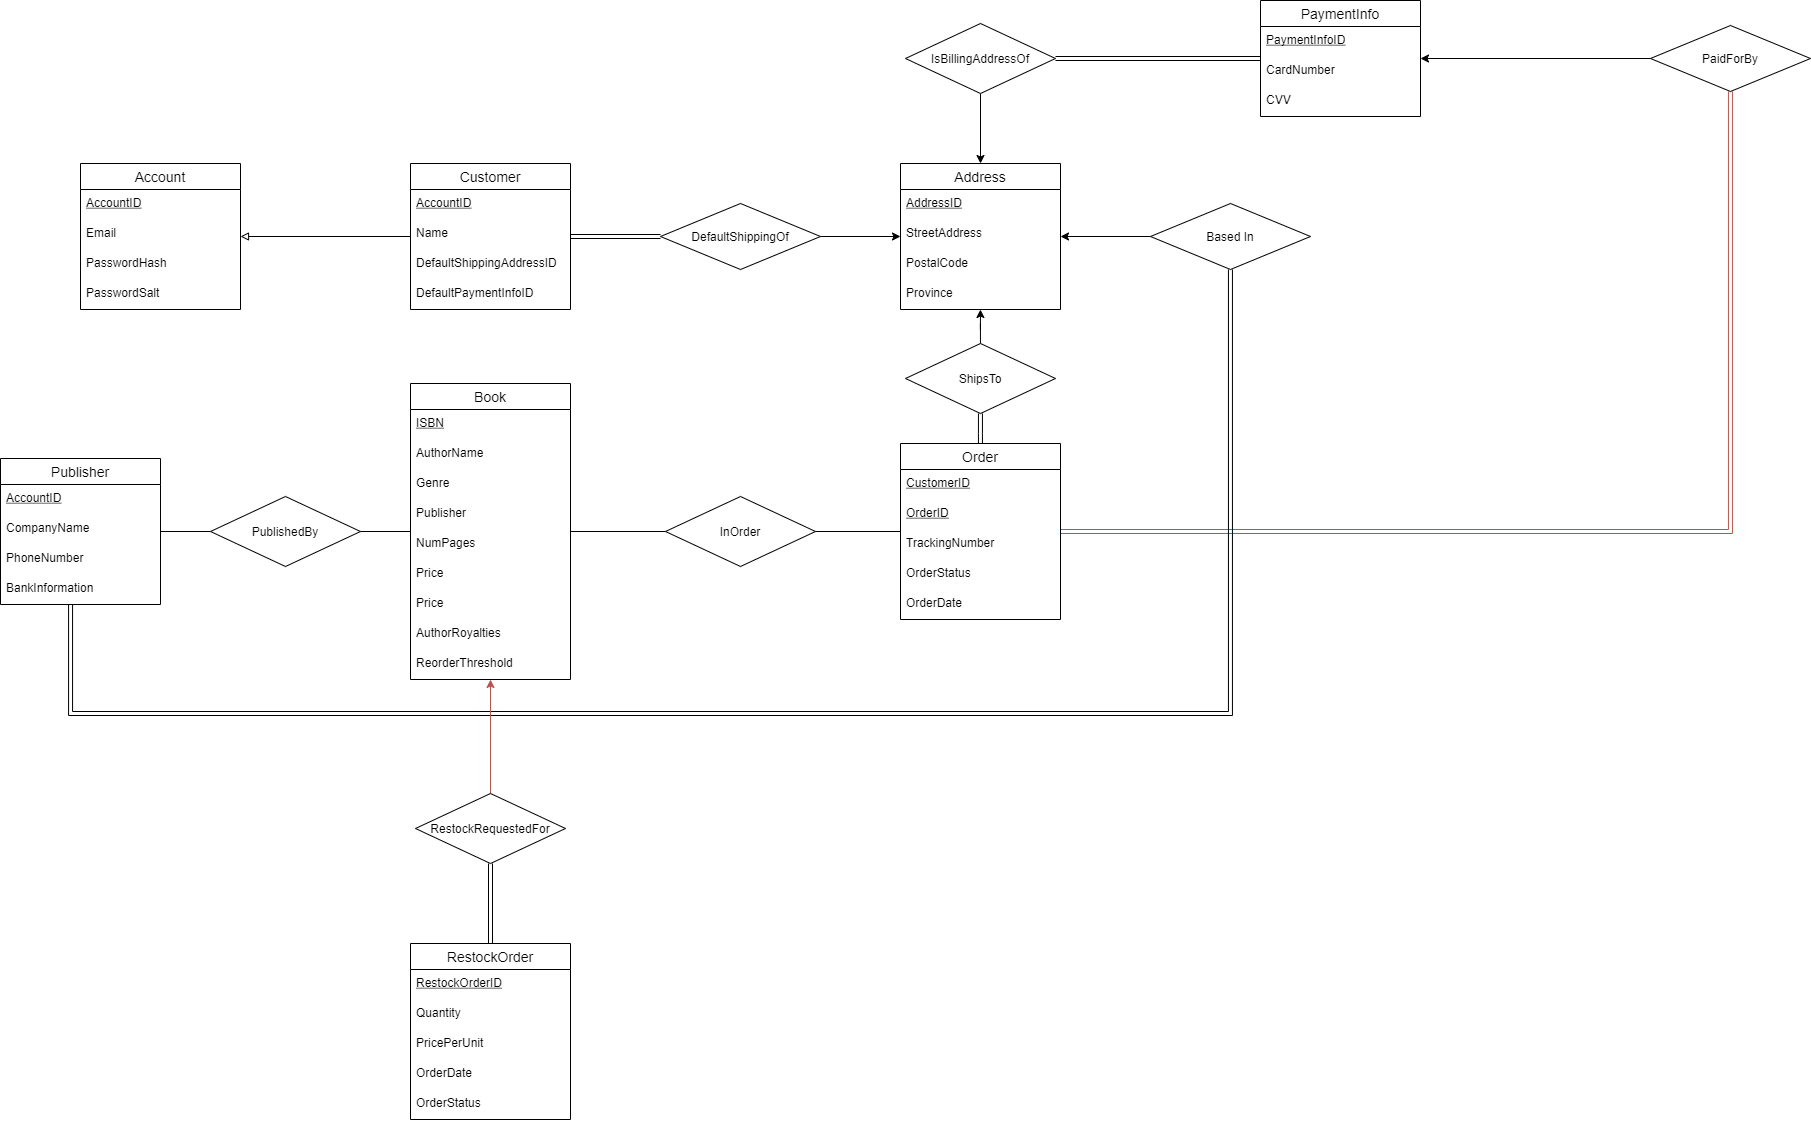
\includegraphics[height=\textwidth]{er}
\end{landscape}

\section{Relations Schema}
The above ER diagram can be broken down into the relation schema below. Primary keys are denoted by underscores. Foreign keys are denoted in italics.
\begin{itemize}
  \item \schema{book}{\pkey{isbn}, title, author_name, genre, publisher, num_pages, price, author_royalties, reorder_threshold, \fkey{publisher_id}}
  \item \schema{address}{\pkey{address_id}, street_address, postal_code, province}
  \item \schema{customer}{\pkey{customer_id}, name, email, password_hash, password_salt, \fkey{default_shipping_address_id, default_payment_info_id}}
  \item \schema{payment_info}{\pkey{payment_info_id}, name_on_card, expiry, card_number, cvv, \fkey{billing_address}}
  \item \schema{publisher}{\pkey{publisher_id}, company_name, phone_number, bank_information, \fkey{address_id}}
  \item \schema{order}{\pkey{order_id}, \fkey{customer_id, shipping_address}, tracking_number, order_status, order_date, \fkey{payment_info_id}}
  \item \schema{in_order}{\fkey{\pkey{isbn, order_id}}, quantity}
  \item \schema{restock_order}{\pkey{restock_order_id}, \fkey{isbn}, quantity, price_per_unit, order_date, order_status}
  \item \schema{in_cart}{\fkey{\pkey{isbn, customer_id}}, quantity}
  \item \schema{owner}{\pkey{owner_id}, name, email, password_hash, password_salt}
  \item \schema{book_collection}{\pkey{collection_id}, \fkey{curator_owner_id}}
  \item \schema{in_collection}{\fkey{\pkey{collection_id, isbn}}}
\end{itemize}

\section{Functional Dependencies}
\begin{itemize}
  \item ISBN \trightarrow{} Title, AuthorName, Genre, Publisher, NumPages, Price, AuthorRoyalties, ReorderThreshold, PublisherAccountID
  \item AddressID \trightarrow{} StreetAddress, PostalCode, Province
  \item CustomerID \trightarrow{} CustomerName, CustomerEmail, CustomerPasswordHash, CustomerPasswordSalt, DefaultShippingAddressID, DefaultPaymentInfoID
  \item PaymentInfoID \trightarrow{} NameOnCard, ExpiryDate, CardNumber, CVV, BillingAddressID
  \item PublisherID \trightarrow{} CompanyName, PhoneNumber, BankInformation, AddressID
  \item OrderID \trightarrow{} CustomerID, TrackingNum, OrderStatus, OrderDate, ShippingAddressID, PaymentInfoID
  \item OrderID, BookISBN \trightarrow{} OrderQuantity
  \item CustomerID, BookISBN \trightarrow{} CartQuantity
  \item RestockOrderID \trightarrow{} BookISBN, Quantity, PricePerUnit, OrderDate, OrderStatus
  \item OwnerID \trightarrow{} OwnerName, OwnerEmail, OwnerPasswordHash, OwnerPasswordSalt
  \item BookCollectionID \trightarrow{} OwnerID
\end{itemize}

\end{document}
